\chapter{Future Works and Conclusion}\label{chap:conclusion}
\section{Integer Quantum Hall Effects}\label{sec:IQHE}
In a \ac{2DES} there are a number of interesting phenomena that occurs at low temperatures in the presence of strong magnetic fields. One such effect is the \ac{IQHE}. The \acs{IQHE} was discovered in 1980 by Klitzing \emph{et al.} \cite{Klitzing_PhysRevLett1980}. They showed that under a quantum regime of temperature and magnetic field there is a quantization of the Hall resistance, which deviates from its linearity in the magnetic field seen in the classical Hall effect, displaying plateaus at particular values of the magnetic field where the Hall resistance is given purely in terms of universal constants. In addition, the plateaus observed in the Hall resistance are accompanied by a vanishing longitudinal resistance \cite{Klitzing_PhysRevLett1980,Ando_RevModPhys1982,Goerbig_2009,Hook_Solid1991}.

\subsection{Theoretical Background}\label{subsec:IQHE_theory}
\begin{figure}[ht]
	\centering
	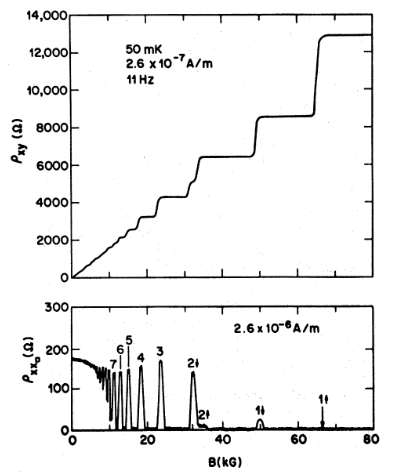
\includegraphics[height=7cm,width=5cm]{figs/future/IQHE_data_RHOxy_RHOxx}
	\caption[Example data of the Integer Quantum Hall Effect]{$\rho_{xx}$ and $\rho_{xy}$ as a function of magnetic field $B$ at low temperature ($T=50\unita{mK}$). The numbers and arrows above the $\rho_{xx}$ maxima refer to the Landau quantum number and the spin polarization of the levels. Figure originally appeared in ref.~\cite{Paalanen_PhysRevB1982}.}
	\label{fig:IQHE_data}
\end{figure}

\subsection{Implementation and Measuring the Integer Quantum Hall Effect}\label{subsec:IQHE_measure}

\section{Shubnikov-de Haas Oscillations}\label{sec:sdh_oscillations}

\section{Limitations}\label{sec:limitations}